\documentclass[conference]{IEEEtran}
\IEEEoverridecommandlockouts
\usepackage{cite}
\usepackage{amsmath,amssymb,amsfonts}
\usepackage{algorithmic}
\usepackage{graphicx}
\usepackage{textcomp}
\usepackage{xcolor}
\usepackage{xcolor}
\usepackage{multirow}
\usepackage{hyperref}
\hypersetup{%
  colorlinks=false,
  urlbordercolor=red
}
\usepackage{subcaption}

\newcommand{\code}[1]{\texttt{#1}}

\def\BibTeX{{\rm B\kern-.05em{\sc i\kern-.025em b}\kern-.08em
    T\kern-.1667em\lower.7ex\hbox{E}\kern-.125emX}}
\begin{document}

\title{Scalable and Cloud programming - Co-Purchase-Analysis Technical Report}

\author{
\IEEEauthorblockN{1\textsuperscript{st} Michele Dinelli}
\IEEEauthorblockA{\textit{dept. of Computer Science and Engineering, University of Bologna}}
}

\maketitle

\begin{abstract}
This document is the technical report for the scalable and cloud programming project developed for the university course held in Bologna (a.y 24/25). Source code is available online as a \href{https://github.com/micheledinelli/scalable-cloud-programming}{GitHub repository}.
\end{abstract}

\begin{IEEEkeywords}
cloud programming, scala, apache spark, google cloud platform, dataproc
\end{IEEEkeywords}

\section{Introduction}
This document is a technical report that describes the implementation and scaling evaluation of a co-purchase-analysis script written in Scala. The system is required to read purchases data from a dataset \cite{dataset} and it must identify co-purchased products by calculating, for each pair of products, the number of orders in which they were purchased together.

\section{Implementation}
The solution used Apache Spark \cite{10.1145/2934664} and runs on distributed nodes using DataProc. Versions used are Scala 2.12.18 and Spark 3.5.5. Implementation follows the map-reduce approach with an eye to scaling efficiency.

\begin{table}[htbp]
\caption{Dataset Format}
\begin{center}
\begin{tabular}{|c|c|}
\hline
\textbf{Order ID}& \textbf{Product ID}\\
\hline
2& 33120 \\
\hline
2&28985 \\ 
\hline
2& 9327 \\
\hline
$\vdots$& \vdots \\
\hline
3421083& 5020 \\
\hline
\end{tabular}
\label{tab:dataset}
\end{center}
\end{table}

First the input is read and mapped to a \code{RDD[T]}. Resilient Distributed Dataset (RDD) are distributed data structures that are accessible as one entity but are shared across nodes. In this case we store couples of \code{Int} values in the RDD (\code{RDD[(Int, Int)]}). This comes from the fact that the dataset consists of rows in the format presented in Table \ref{tab:dataset}.

After reading the input, the dataset is partitioned across nodes using a \code{HashPartitioner}. This partitioner assigns each key-value pair to a partition based on the hash of the key. Specifically, a pair (key, value) is sent to the partition with index:

\begin{equation}
    \texttt{hash}(key) \mod n
\end{equation}

where $\texttt{hash}(key)$ is an hash function on the key and $n$ is the number of partitions. This ensures that all pairs with the same key end up in the same partition (and thus on the same node), which is crucial for operations like \code{groupByKey} to work correctly without requiring additional shuffling.

Data are then grouped by order identifier, producing a \code{RDD[(Int, Iterable[Int])]} where the key is the order identifier. This is done using \code{groupByKey} which is an operation that triggers shuffling, but since the dataset was previously partitioned using a \code{HashPartitioner} based on the same key (order ID), all entries with the same key are already co-located in the same partition. As a result, the shuffle still occurs but is significantly optimized.

Next, for each grouped order, the list of product IDs is converted to a distinct list to remove duplicates. All unique pairs of products $(i,j)$ such that $i<j$ are generated from this list, and each pair is associated with the value 1. This results in a new RDD of the form \code{RDD[((Int, Int), 1)]}, representing one co-purchase occurrence per pair.

Finally, all identical product pairs are aggregated using \code{reduceByKey}, summing the counts to compute the total number of times each pair was co-purchased. The results are formatted and written to the output directory using \code{saveAsTextFile}. A \code{coalesce(1)} is used to write the result into a single output file.

\begin{figure}[htbp]
\centerline{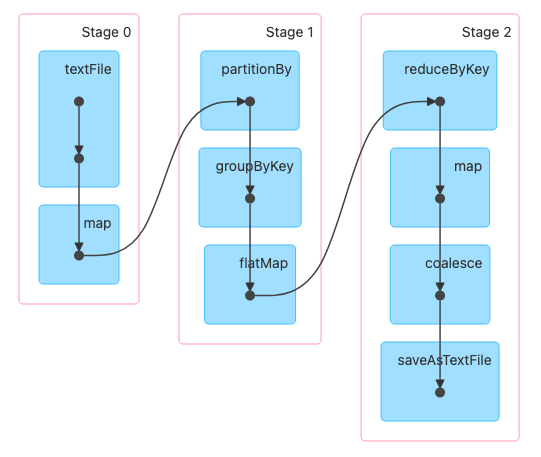
\includegraphics[width=0.5\linewidth]{dag.png}}
\caption{DAG of the implemented solution}
\label{fig:dag}
\end{figure}

The steps are represented as a Directed Acyclic Graph (DAG) (Fig. \ref{fig:dag}) produced by the SparkUI.

\section{Analytical Metrics}

\subsection{Speedup}
We define $T(n)$ as the execution time of a parallel program with $n$ nodes. The speedup $S(n)$ is defined by the formula
\begin{equation}
S(n)= \frac{T(1)}{T(n)} 
\end{equation}
Ideally, the program with $n$ nodes requires $1/n$ the time of the program with 1 node. $S(n) = n$ is a linear speedup but in practice it's sublinear $S(n) \leq n$. This limitation is captured by Amdahl's Law \cite{10.1145/1465482.1465560}, which states that if a task consists of a fraction $f$ hat is inherently sequential (i.e., cannot be parallelized), and the remaining fraction $1-f$ can be sped up by a factor of $P$ then the maximum achievable speedup is
\begin{equation}
\frac{1}{f + \frac{1-f}{P}}\label{eq:amdahl} < \frac{1}{f}
\end{equation}
Even if we could infinitely speed up the parallelizable part (i.e., $P \rightarrow \infty$), the overall speedup would still be limited by the sequential portion $f$.

\subsection{Scaling Efficiency}
To evaluate the impact of Amdahl's law \eqref{eq:amdahl} on a distributed system we introduce Strong Scaling Efficiency (SSE) and Weak Scaling Efficiency (WSE).

\subsubsection{SSE} measures how increasing the number of nodes impacts the speedup while keeping the total amount of work fixed. $SSE$ is defined by
\begin{equation}
    SSE(n) = \frac{S(n)}{n} = \frac{T(1)}{n T(n)}
\end{equation}
The total amount of work remains constant, while the amount of work for each processor decreases as $n$ increases. SSE is limited by the constant $\frac{1}{f}$ so it tends to zero.
\begin{equation}
    \lim_{n\to\infty} SSE(n) = \lim_{n\to\infty} \frac{T(1)}{n T(n)} = \lim_{n\to\infty} \frac{1}{fn} = 0
\end{equation}

% \subsubsection{WSE} measures how productively a program uses added resources and is defined by
% \begin{equation}
%     WSE(n) = \frac{T_1}{T_n}
% \end{equation}
% Where $T_i$ is time required to complete $i$ work unit/s with $i$ node/s. WSE increases the number of nodes $n$ keeping the per-node work fixed as the total amount of work grows as $n$ increases.

\section{Local Results}
Local testing was done on an Apple Mac Mini with an Apple M4 chip (10-core CPU: 4 performance cores, 6 efficiency cores; 10-core GPU; 120GB/s memory bandwidth; 16GB unified memory). The code was compiled and packaged using sbt, a build tool for Java and Scala. 

To get a sense of how the program scales, tests were run locally by gradually increasing the number of cores available to Spark. The resulting Jar, when submitted to Spark, produces the following results:

\begin{table}[htbp]
\caption{Local Results}
\begin{center}
\begin{tabular}{|c|c|c|}
\hline
\textbf{Number of Cores}& \textbf{Partitions} & \textbf{Time (min)}\\
\hline
1& 2& 5,5\\
\hline
2& 4& 4,3\\
\hline
4& 8& 3,0\\
\hline
8& 16& 2,5\\
\hline
10& 30& 2,3\\
\hline
\end{tabular}
\label{tab:local-results}
\end{center}
\end{table}

The full list of run is shown in Fig. \ref{fig:local-testing}. Results are not sorted.

For local testing we notice that the Speedup is sublinear since for $n=10$

\begin{equation}
    S(n) = \frac{T(1)}{T(n)} = \frac{5.5}{2.3} \approx 2.39
\end{equation}

And SSE for $n=10$ is 

\begin{equation}
    SSE(n) = \frac{T(1)}{nT(n)} = \frac{5.5}{n 2.3} \approx 0,239
\end{equation}

This gave a rough idea of how the system handles parallel execution. However, since everything runs on the same machine, it doesn't reflect the full complexity of a real distributed setup. For example there’s no network delay or data transfer between nodes.

\section{Results}
Final testing was done using Google Cloud Dataproc. The Jar produced and the input file have been stored in a bucket and then a Spark Job was submitted increasing workers from 1 to 4. Results are shown in Table \ref{tab:results}.

% \renewcommand{\arraystretch}{1.2}
% \begin{table}[htbp]
% \caption{Results}
% \begin{center}
% \begin{tabular}{|c|c|c|c|c|}
% \hline
% \textbf{Workers (n)}& \textbf{Time (s)}& \textbf{S(n) (ratio)}& \textbf{SSE(n)}& \textbf{Machine}\\
% \hline
% 1& 734,09& \slash& \slash& \multirow{7}{*}{n2-standard-4} \\
% \cline{1-4}
% \multirow{2}{*}{2}  & 322,55& 2,275& 1,137& \\
% \cline{2-4}
%                     & 322,42& 2,279& 1,139& \\
% \cline{1-4}
% \multirow{2}{*}{3}  & 205,61& 3,570& 1,19& \\
% \cline{2-4}
%                     & 211,32& 3,473& 1,157& \\
% \cline{1-4}
% \multirow{2}{*}{4}  & 176,36& 4,162& 1,04& \\
% \cline{2-4}
%                     & 167,40& 4,385& 1,096&  \\
% \hline
% \end{tabular}
% \label{tab:results}
% \end{center}
% \end{table}

\renewcommand{\arraystretch}{1.2}
\begin{table}[htbp]
\caption{Results}
\begin{center}
\begin{tabular}{|c|c|c|c|c|}
\hline
\textbf{Workers (n)}& \textbf{Time (s)}& \textbf{S(n) (ratio)}& \textbf{SSE(n)}& \textbf{Machine}\\
\hline
1& 753& \slash& \slash& \multirow{7}{*}{n2-standard-4} \\
\cline{1-4}
\multirow{2}{*}{2}  & 337& 2,23& 1,11& \\
\cline{2-4}
                    & 336& 2,24& 1,12& \\
\cline{1-4}
\multirow{2}{*}{3}  & 222& 3,39& 1,13& \\
\cline{2-4}
                    & 226& 3,33& 1,11& \\
\cline{1-4}
\multirow{2}{*}{4}  & 195& 3,86& 0.96& \\
\cline{2-4}
                    & 181& 4,16& 1,04& \\
\hline
\end{tabular}
\label{tab:results}
\end{center}
\end{table}

The results turned out quite encouraging, showing that the solution scales well as more workers are added. Speedup and efficiency remained strong up to four nodes, which suggests that the workload benefits from parallel execution. That said, Amdahl’s Law reminds us that this improvement won’t continue forever, there’s a point where adding more workers won’t help much due to the parts of the task that can’t be parallelized. The n2-standard-4 machines performed very good and seem like a goof choice for future tests. Unfortunately, we couldn’t explore beyond this setup due to limited Google Cloud credits.

The product pair with the highest number of co-purchases is (13176, 47209), appearing together 62.341 times.

\bibliographystyle{IEEEtran}
\bibliography{bib}

\section*{Appendix}

\begin{figure}[htpb]
    \centering
    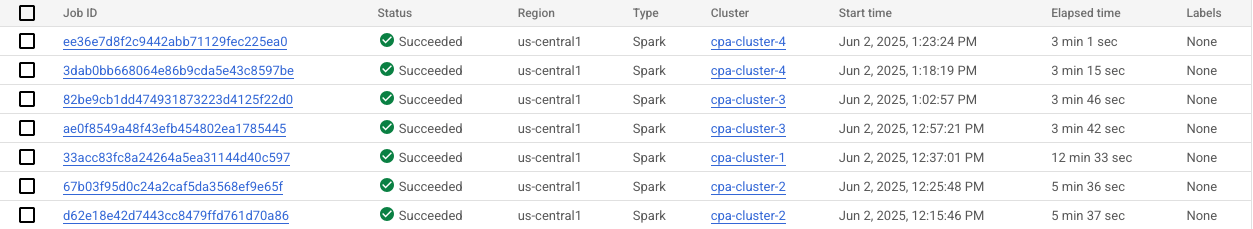
\includegraphics[width=\linewidth]{dataproc-testing.png}
    \caption{Dataproc testing results}
    \label{fig:dataproc-testing}
\end{figure}

\begin{figure}[htpb]
  \centering
  \begin{subfigure}[b]{0.49\textwidth}
    \centering
    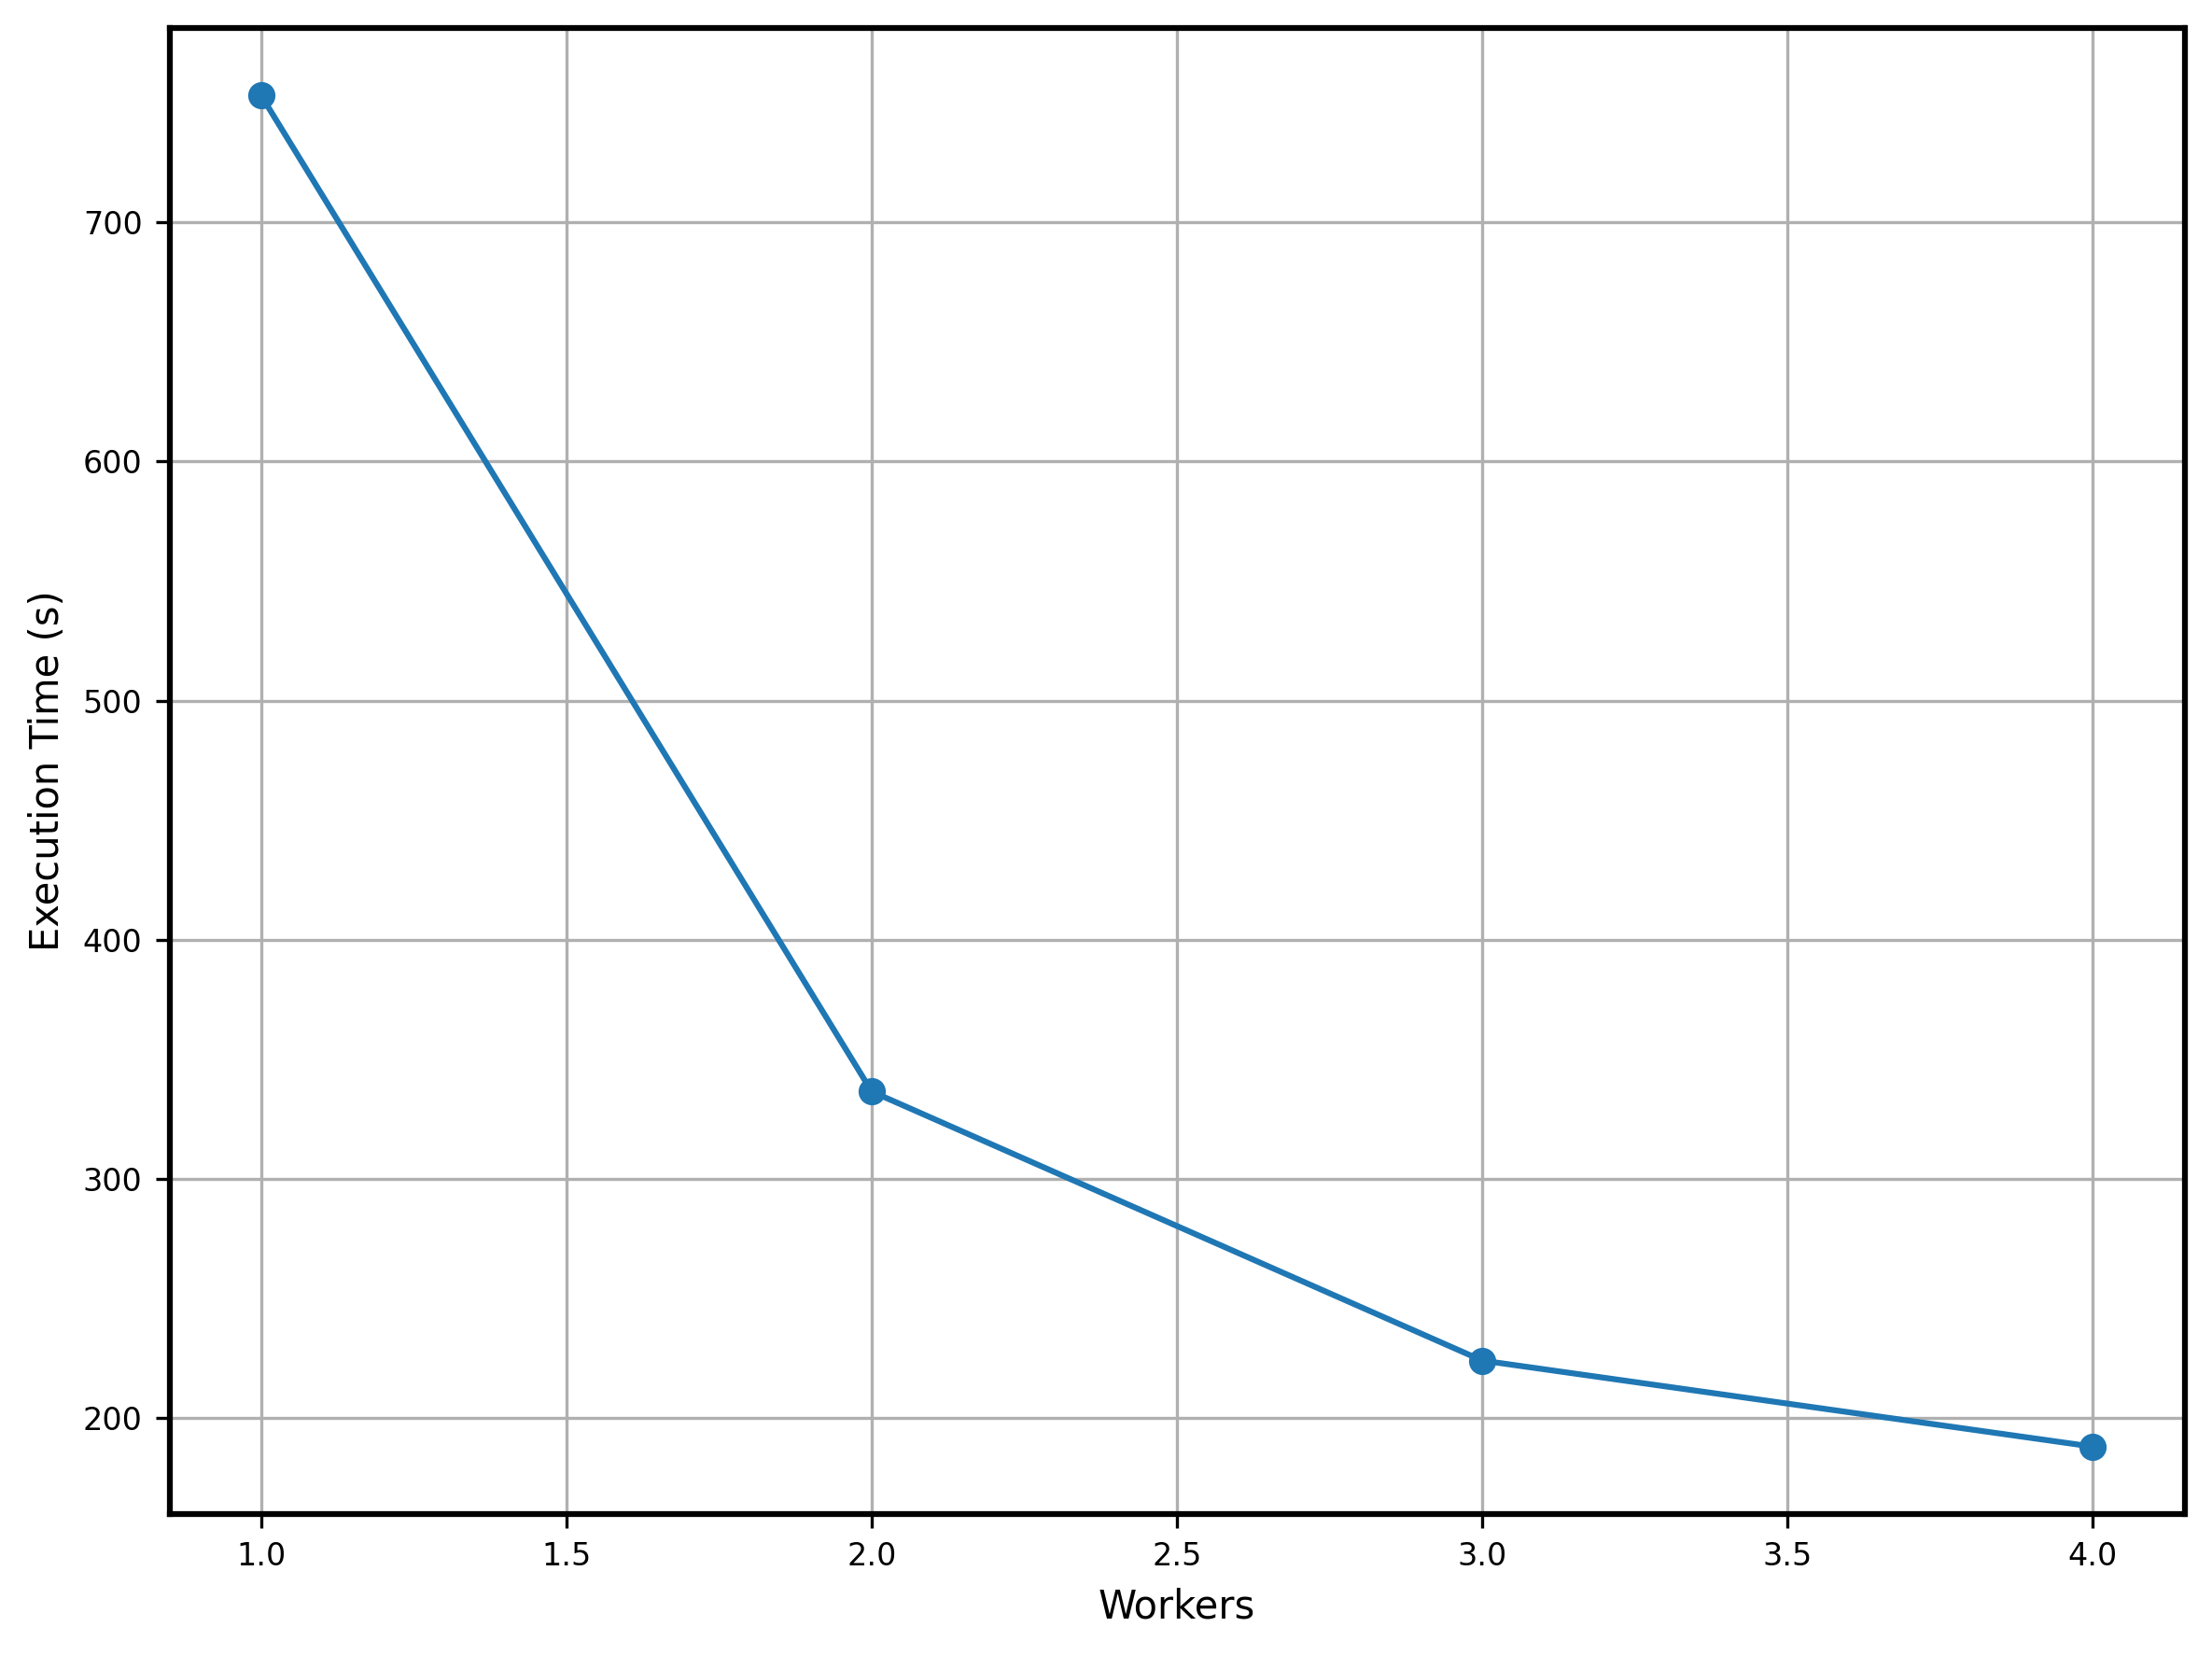
\includegraphics[width=0.7\linewidth]{execution_time.png}
    \caption{Execution Time vs Workers}
    \label{fig:sub1}
  \end{subfigure}
  \hfill
  \begin{subfigure}[b]{0.49\textwidth}
    \centering
    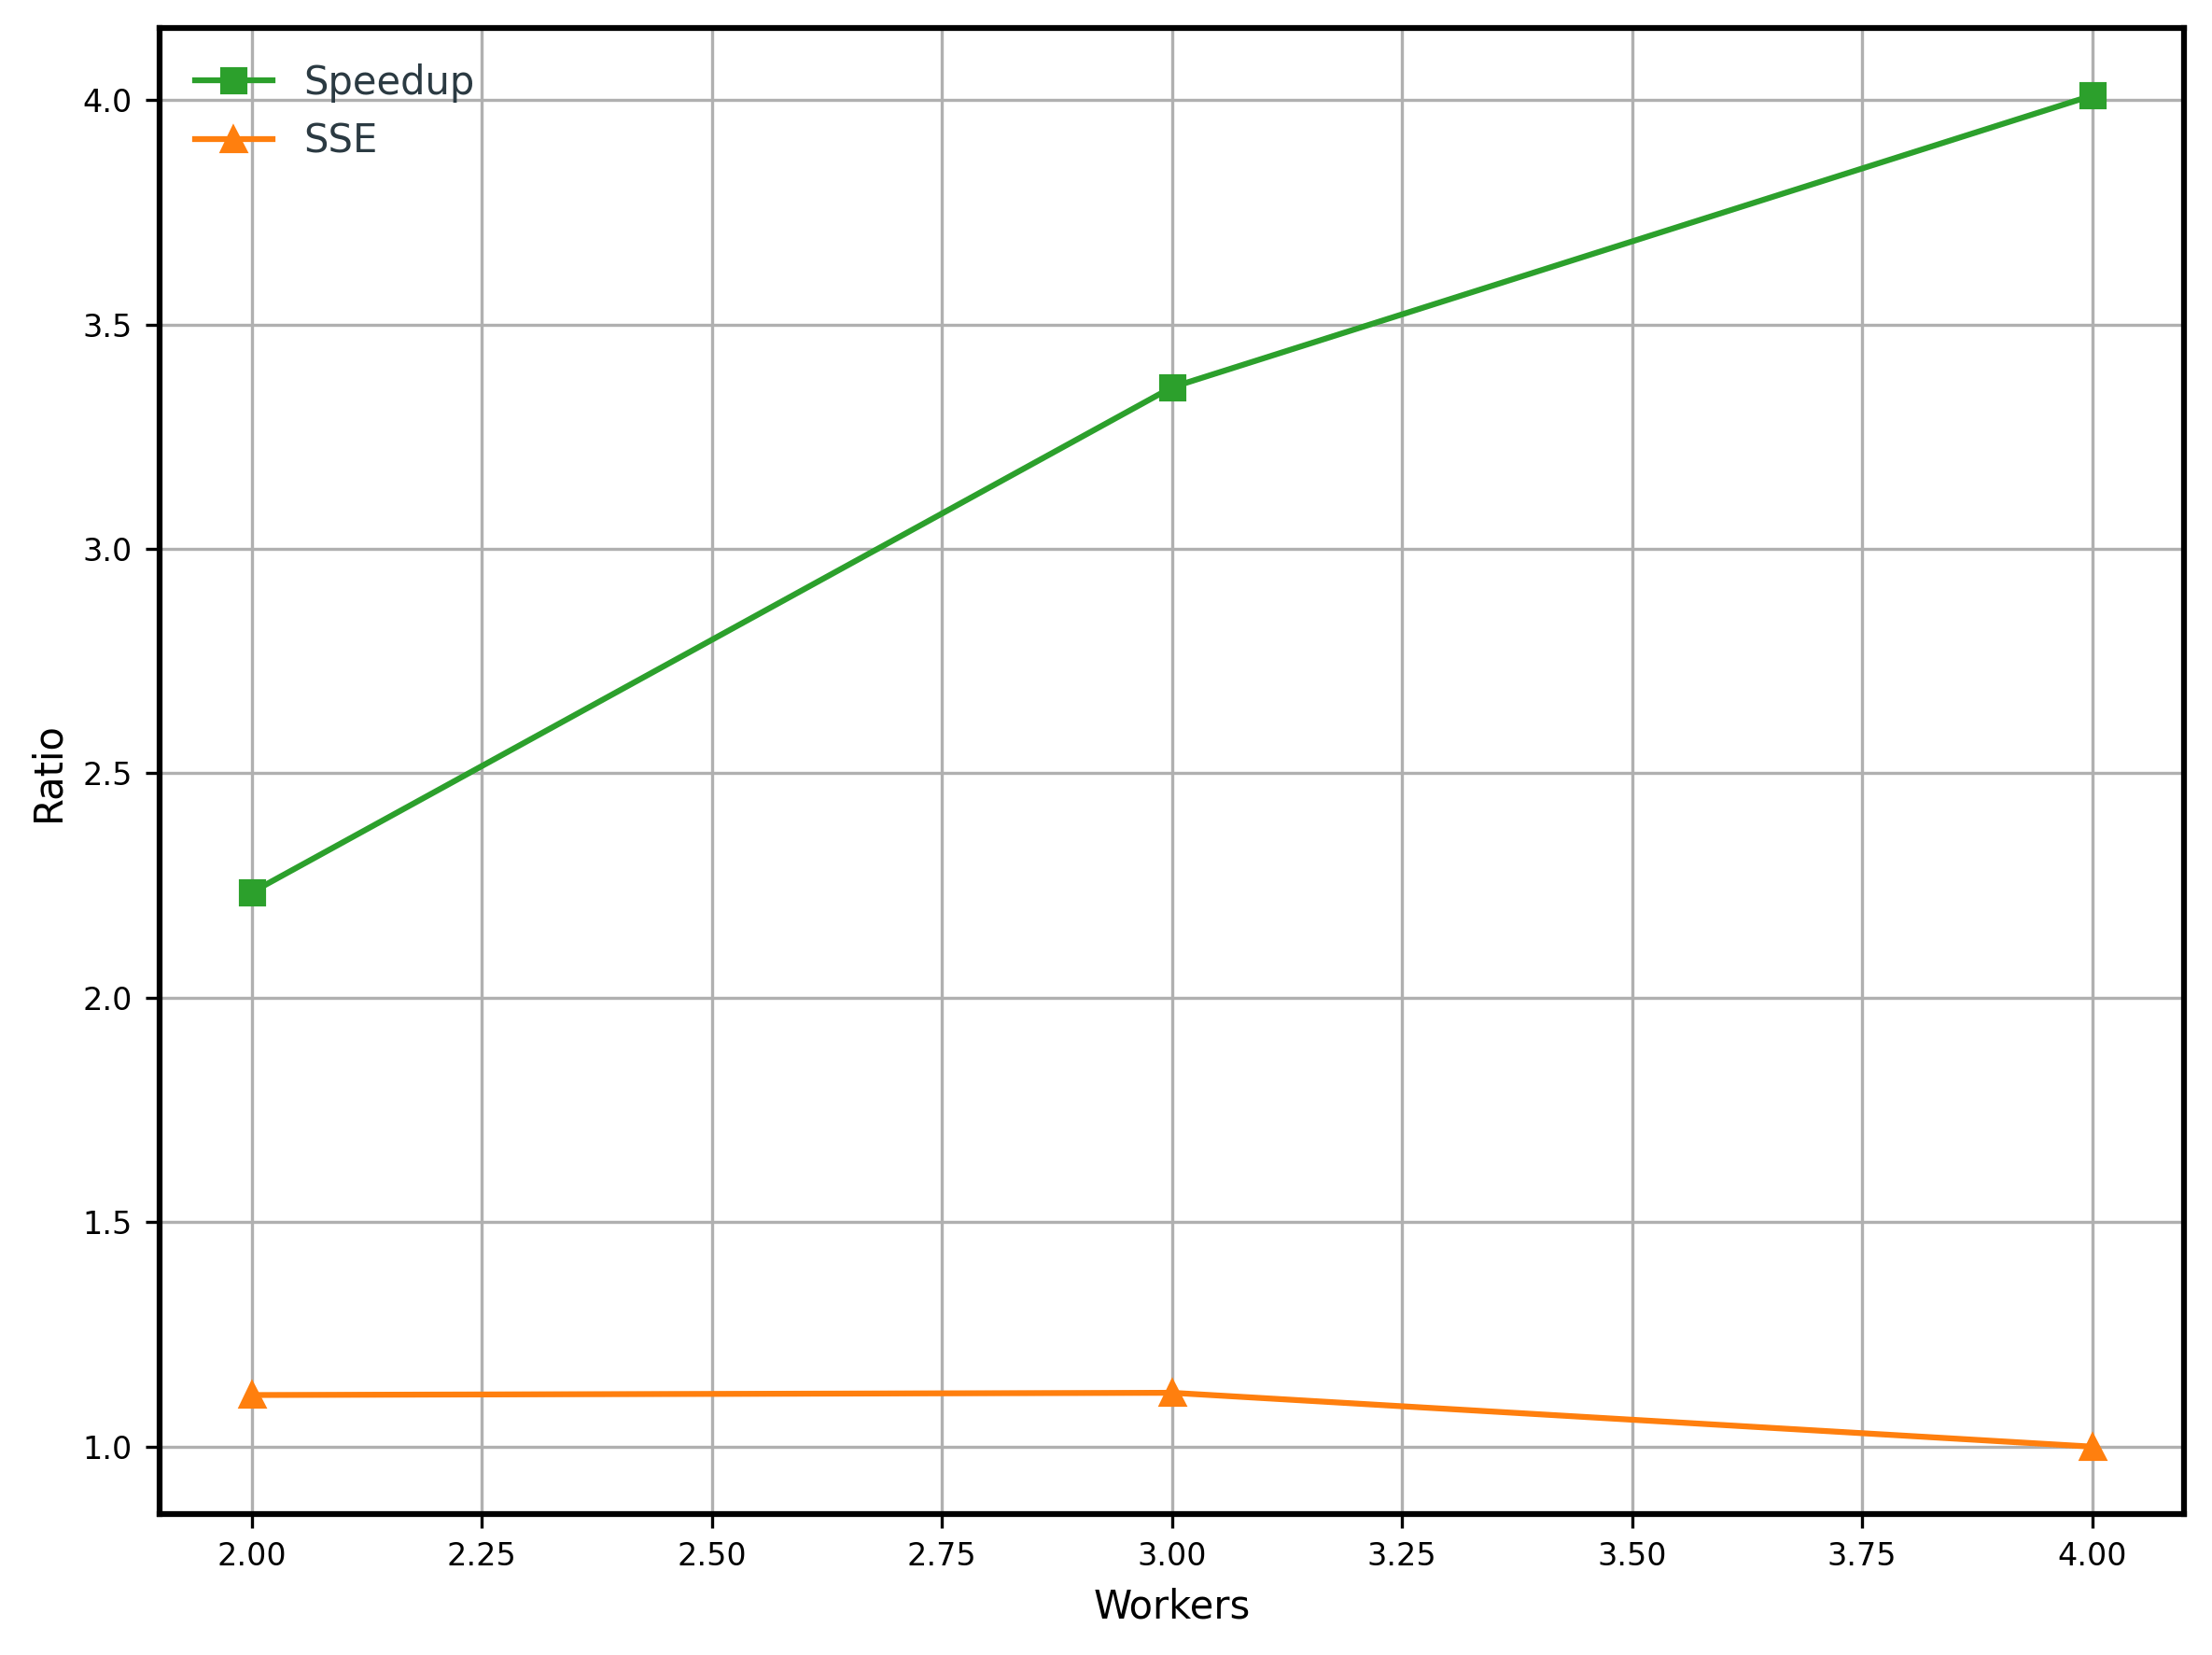
\includegraphics[width=0.7\linewidth]{speedup-sse.png}
    \caption{SpeedUp and SSE vs Workers}
    \label{fig:sub2}
  \end{subfigure}
  \caption{Performance metrics as the number of workers increases. (a) shows execution time vs number of workers. As the number of workers increases, execution time decreases. (b) shows speedup and SSE vs number of workers. While speedup improves with more workers, SSE eventually declines due to Amdahl's law \cite{10.1145/1465482.1465560}.}
  \label{fig:results}
\end{figure}

\begin{figure}[htpb]
    \centering
    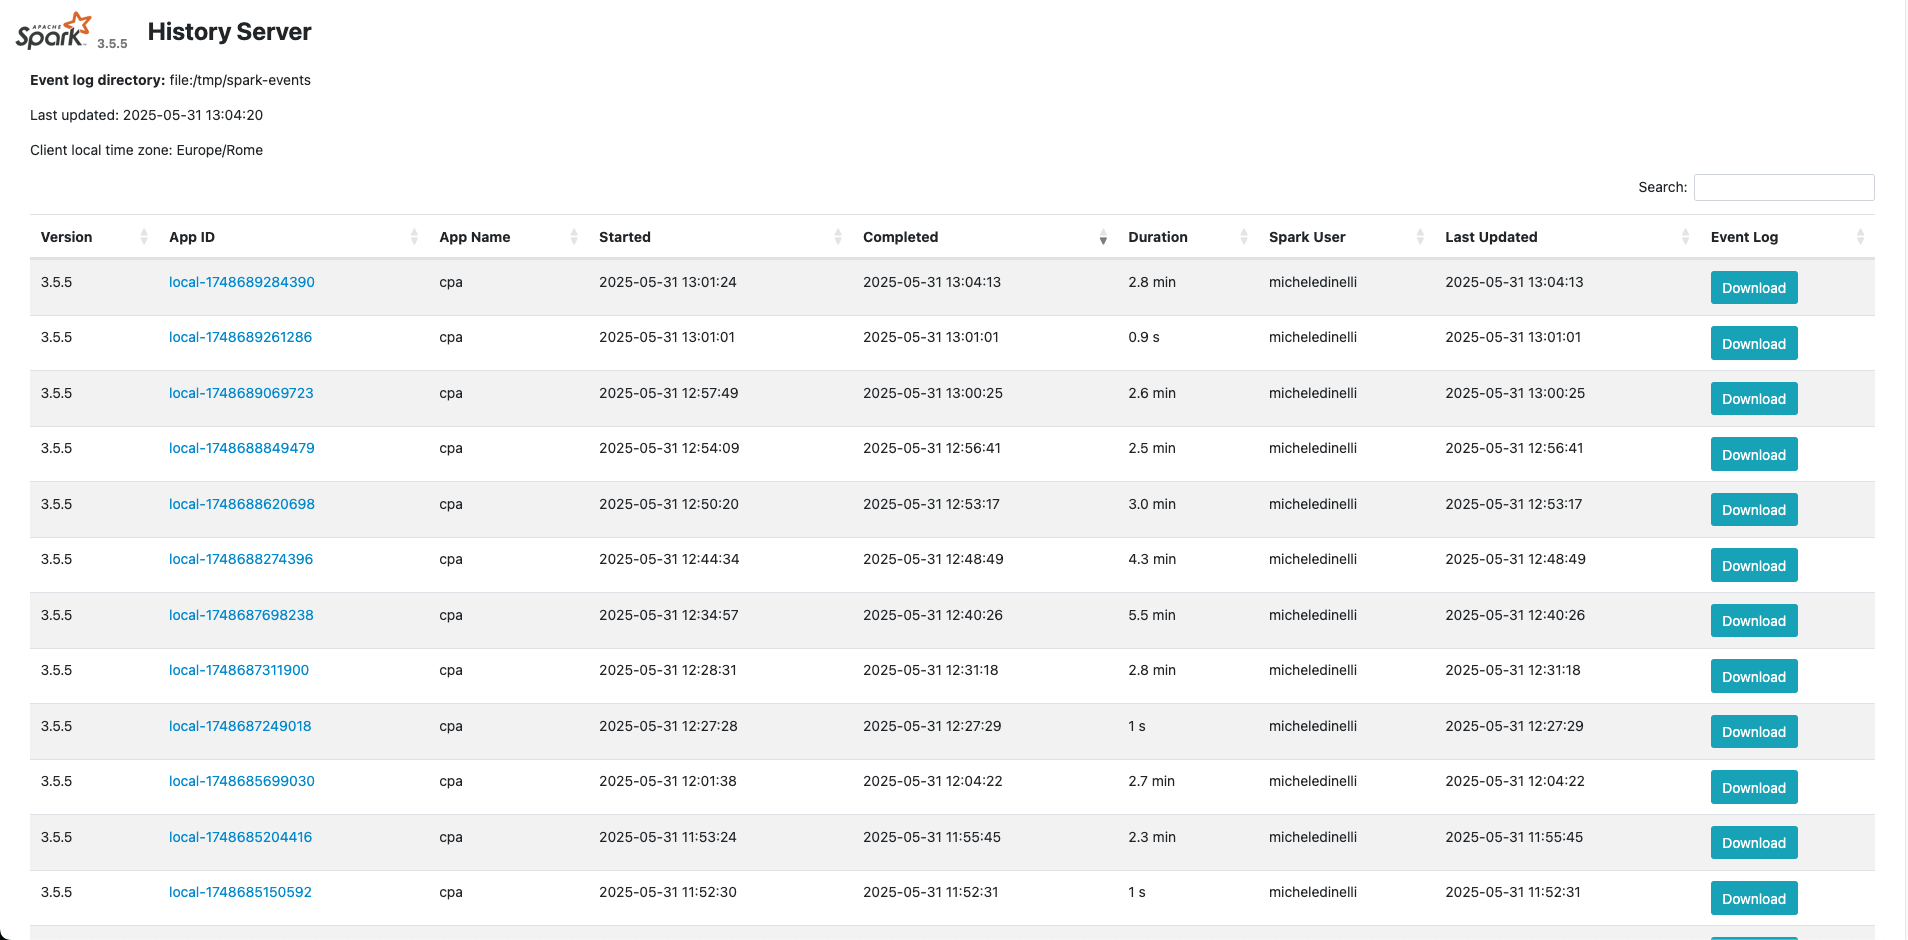
\includegraphics[width=\linewidth]{local-testing.png}
    \caption{Local testing results}
    \label{fig:local-testing}
\end{figure}


\end{document}
